% This is based on the LLNCS.DEM the demonstration file of
% the LaTeX macro package from Springer-Verlag
% for Lecture Notes in Computer Science,
% version 2.4 for LaTeX2e as of 16. April 2010
%
% See http://www.springer.com/computer/lncs/lncs+authors?SGWID=0-40209-0-0-0
% for the full guidelines.
%

\documentclass{llncs}

\usepackage[utf8]{inputenc}
\usepackage[T1]{fontenc}
\usepackage[polish]{babel}
\usepackage[colorinlistoftodos]{todonotes}
\usepackage{hyperref}
\usepackage{subfig}

\begin{document}

\title{Konwolucyjna sieć neuronowa grająca w Connect4}
%
\titlerunning{ConvConnect4}  % abbreviated title (for running head)
%                                     also used for the TOC unless
%                                     \toctitle is used
%
\author{Tomasz Janiszewski\inst{1} \and Jakub Dutkowski\inst{2}}
%
\authorrunning{Tomasz Janiszewski, Jakub Dutkowski} % abbreviated author list (for running head)
%
%%%% list of authors for the TOC (use if author list has to be modified)
\tocauthor{Tomasz Janiszewski and Jakub Dutkowski}

\institute{Politechnika Warszawska\\
Wydział Matematyki i Nauk Informacyjnych
\email{janiszewskit@student.mini.pw.edu.pl}~~
\email{dutkowskij@student.mini.pw.edu.pl}}

\maketitle              % typeset the title of the contribution

\keywords{Connect4, Convolutional Neural Network, Deep learning, cognitive approach,
intuitive playing, human-like problem solving, example-based learning, Connect Four.}
%
\section{Wstęp}
Celem projektu jest stworzenie rozwiązania znajdującego optymalny ruch (bądź jego przybliżenie) w grze Connect Four (\emph{pol. Czwórki}) \cite{connect4:wiki} na podstawie obrazu planszy, bez przeszukiwania drzewa gry. 
Rozwiązanie zostanie zbudowane w oparciu o konwolucyjną sieć neuronową.

\section{Reprezentacja planszy}
Aby wykorzystać lokalność kontekstu gry, plansza do gry podzielona będzie na nachodzące na siebie sektory - kwadraty $4x4$ (jak na \autoref{fig:C4Podzial}). 
Każdy z kwadratów reprezentowany będzie jako wektor szesnastu liczb $\{-1, 0, 1\}$, gdzie:
\begin{description}
	\item[1] oznacza krążęk gracza aktywnego
	\item[-1] oznacza krążek gracza nieaktywnego
	\item[0] oznacza puste pole
\end{description} 

Wartości odpowiadające polom w sektorze ustawione będą kolejno jak na \autoref{fig:C4Kolejnosc}. 

\begin{figure}
	\centering	
	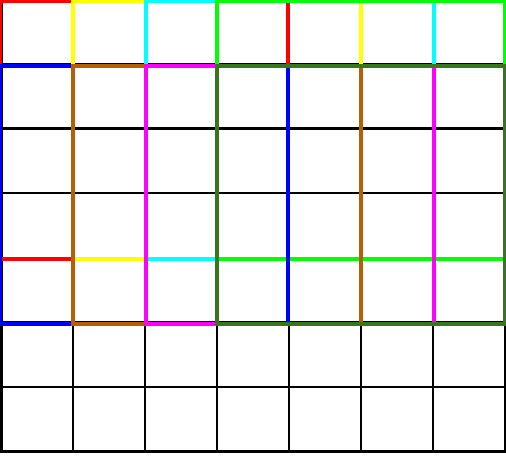
\includegraphics[width=0.5\textwidth]{img/ConnectFour4x4.pdf}
	\caption{Podział planszy na kwadraty 4x4. Dla czytelności, przedstawiono tylko pierwsze dwa wiersze.}
	\label{fig:C4Podzial}
\end{figure}

\begin{figure}
	\centering	
	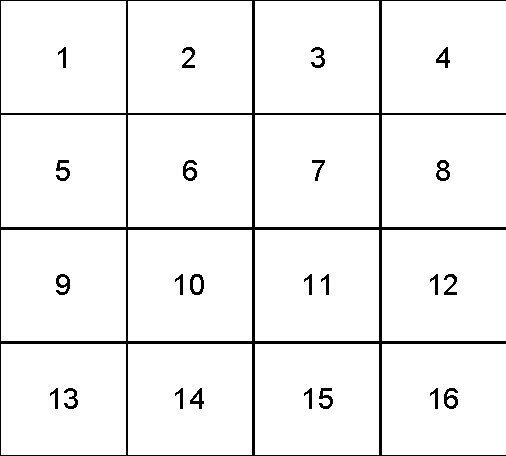
\includegraphics[width=0.5\textwidth]{img/ConnectFourOrder.pdf}	\caption{Kolejność pól w wektorze kodującym sektor planszy.}
	\label{fig:C4Kolejnosc}
\end{figure}

\section{Opis sieci}
Wejście sieci będzie składało się z 9x16 neuronów - po jednym neuronie na każde z 16 pól w każdym z 9 sektorów. Części odpowiadające kolejnym sektorom będą miały związane odpowiednie wagi (np. waga odpowiadająca polu nr 1 w sektorze I będzie związana z wagą pola nr 1 w sektorze nr III). Kolejna warstwa składała się będzie z 4x9 neuronów - po jednym na każdą kolumnę każdego z sektorów
\todo {dodaj jak połączyć te sektory - pionowo?}


Wyjście sieci składało się będzie z siedmiu neuronów odpowiadającym kolumnom na planszy. Największa wartość oznacza numer kolumny w następnym ruchu.

\section{Algorytm uczenia i grania}
Sieć będzie uczona za pomocą algorytmu propagacji wstecznej. Dane treningowe wygenerowane zostaną za pomocą programu Velena\cite{velena} wykonującego perfekcycjne ruchy.

%
% ---- Bibliography ----
%
\begin{thebibliography}{4}
%
\bibitem {mandziuk2011}
Mandziuk, J.:
\textsl{Towards Cognitively Plausible Game Playing Systems}
IEEE COMPUTATIONAL INTELLIGENCE MAGAZINE, Maj, 2011
\bibitem {Ah-Hwee}
Ah-Hwee Tan
\textsl{FALCON: A Fusion Architecture for Learning, COgnition, and Navigation}
\bibitem {webinar}
Yann LeCun
\textsl{Gtc Express Convolutional Networks Webinar}
\url{http://on-demand.gputechconf.com/gtc/2014/webinar/gtc-express-convolutional-networks-webinar.mp4}
\bibitem {connect4:wiki}
\textsl{Connect Four --- {W}ikipedia{,} The Free Encyclopedia}
\url{http://en.wikipedia.org/wiki/Connect_Four}
\bibitem {velena}
\textsl{A Shannon C-type program which plays connect four perfectly}
\url{http://www.ce.unipr.it/~gbe/velena.html}
\end{thebibliography}

\end{document}
